%===================================== CHAP 7 =================================

\chapter{Project Life Cycle}

\section{Planning}
The group initiated the project with a planning and research phase, lasting from January the 11th to February the 3rd. 

The importance of the planning phase was emphasised by the group to avoid being forced to start over because the project was insufficient according to what the customer wanted. \\

The planning phase was initiated by thoroughly choosing the right project, focusing on the strengths and weaknesses within the group. To ensure that every member had the same ambitions and a common understating of what the group expected of each other, a group contract was also formulated. This contract has been important for the group dynamic (see appendix \ref{group_contract}). The risk analysis (see section \ref{riskAnalysis}) was also developed during the planning phase, as issues might arise unexpectedly and needed to be managed in a proper fashion. The risk analysis was used to prevent and mitigate issues as they were to happen.  \\  

As the project was assigned - the group prioritized to establish contact with the customer to get a more precise idea of what was to be developed. A contract between the team and the customer was also formulated - ensuring both parties held the same expectations for the project, and of each other during the development process (see appendix \ref{customer_contract}).\\

As the group achieved a better idea of what the project implied - a set of roles were created. These were delegated to the group members depending on prior experience and wishes (see section \ref{projectOrganisation}).


\begin{figure}[t]
\centering
    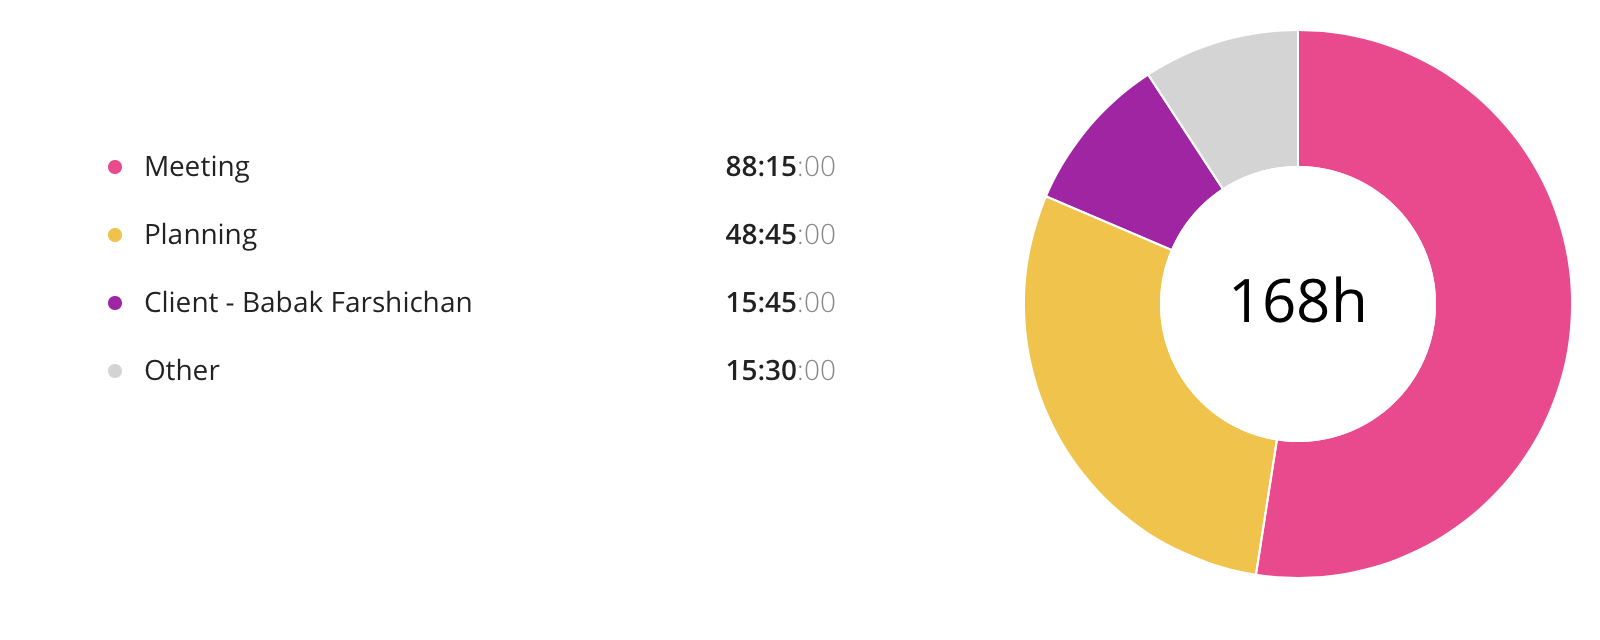
\includegraphics[width=0.55\textwidth]{fig/planning-and-research-diagram}
\caption{Planning and research, hours distributed to work tasks}
\end{figure}


\section{Sprint 0}
\label{sprint0}
The sprint goal for sprint 0 was "Create first design draft, planning and set up product backlog."

Sprint 0 did not have any user stories. Instead the sprint main focus was to set up the workspace; create an index template in Django, create a product backlog with the customer, decide the MVP (see section \ref{MVP}), create a first design draft of the application and doing as much planning as possible. The group chose to do it this way, so the development could start already in the beginning of sprint 1.

The design draft was drawn as a paper prototype (see section \ref{ss:paper_prototype}), and the group performed a demonstration to the customer. He was satisfied with the idea, and it created a great discussion about how the group should continue working.

\subsubsection{Sprint retrospective meeting summary}
The group are satisfied with their own efforts. Heaps of work are accomplished, and everyone are motivated to keep working next week.
    
The group agrees that they should be more effective in their work sessions, so they can accomplish more. To do this it is important that everyone take responsibility of keeping the group on track, and tell if people are not concentrate on the task.

\begin{figure}[ht]
\centering
    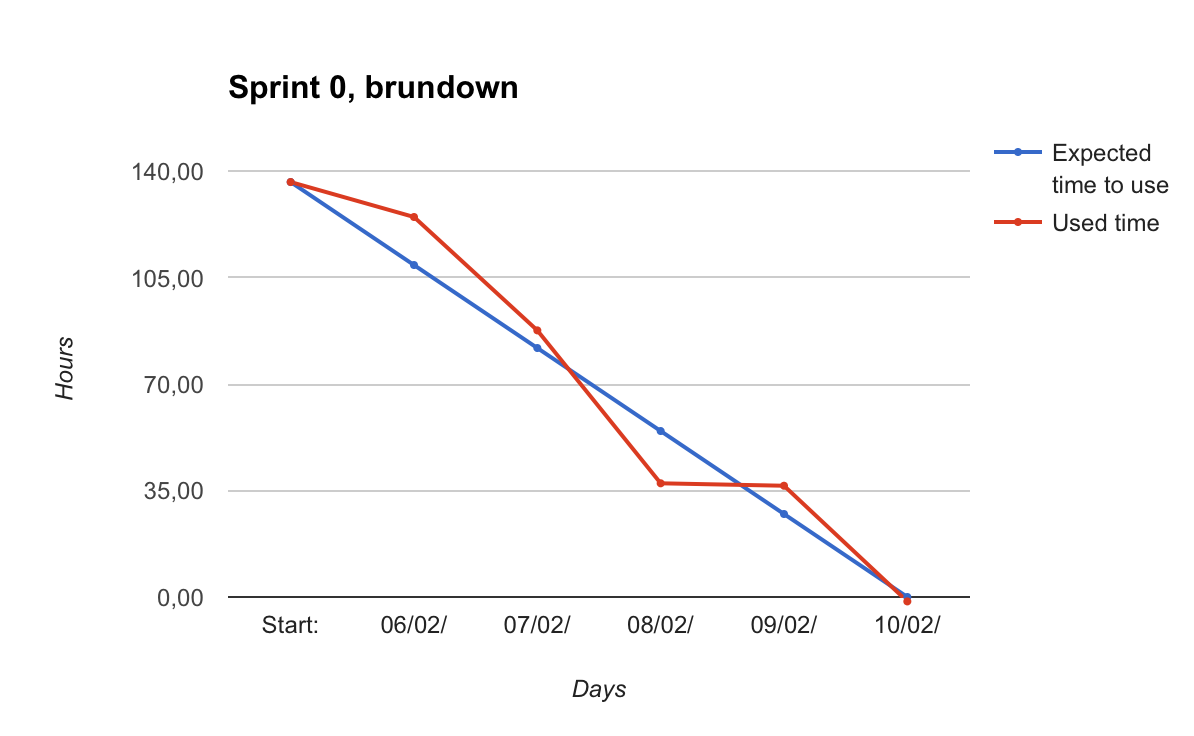
\includegraphics[width=0.8\textwidth]{fig/sprint0}
\caption{Sprint 0, burndown}
\end{figure}

\begin{figure}[ht]
\centering
    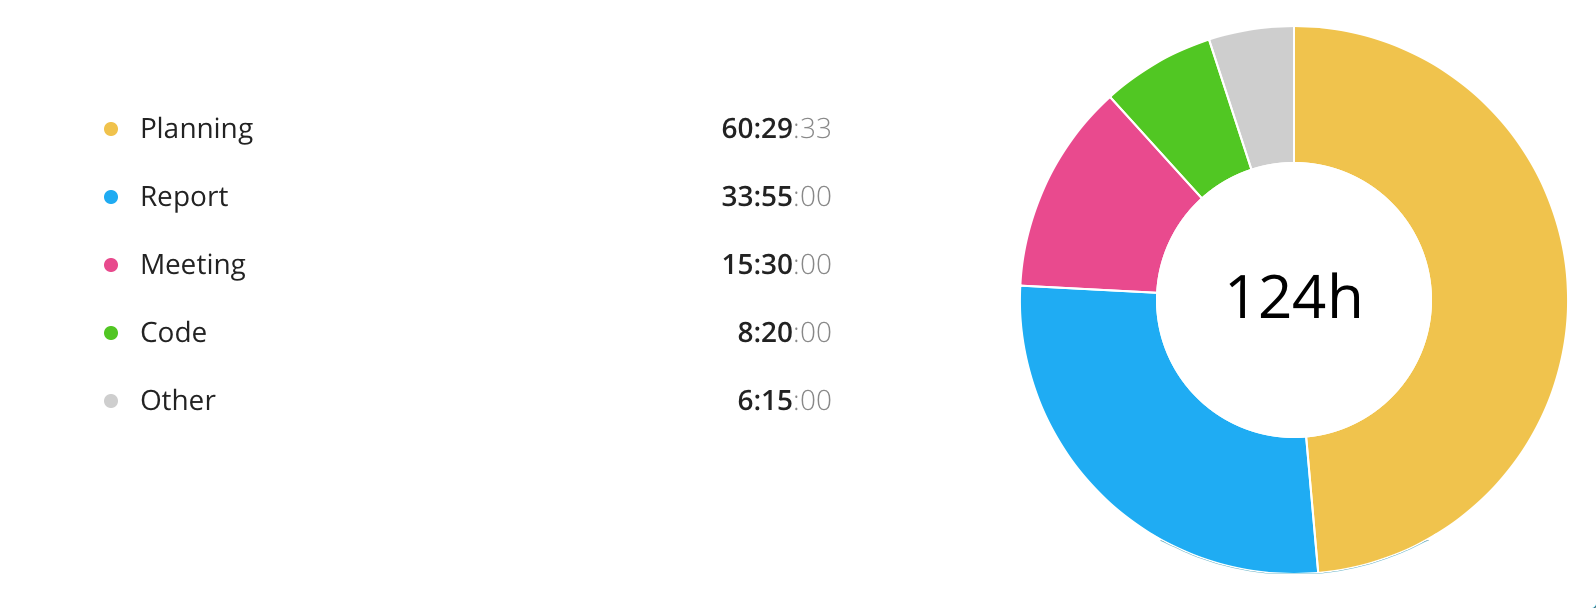
\includegraphics[width=0.8\textwidth]{fig/sprint0-diagram}
\caption{Sprint 0, hours distributed to work tasks}
\end{figure}



\section{Sprint 1}
\label{sprint1}
The overall sprint goal for sprint 1 was to "Deliver first interactive prototype to customer". To achieve this goal, the group created milestones during the sprint planning, that should be finalized during the iteration. The milestones were as as follows:

\begin{itemize}
  \item Create a mock up database.
  \item Create a flow diagram.
  \item Create issues on GitHub.
  \item Make log in, with different GUI for each role (child, parent, activity      provider, maintainer and anonymous).
  \item Log in with Facebook.
  \item Anonymous user should maybe not be able to see who is going to a activity anonymous should not be able to sign up for activity, before the user has logged in.
  \item  Site map Create skeleton for all pages in site map Investigate the possibility of changing the language (create a dynamic page where all words are listed)
  \item Update wiki (to have the flow diagram, site map and user manual)
\end{itemize}
 
Two problems were encountered this sprint. The first one was that one group member asked for five days off to travel. The group concluded this was very inconvenient this early on in the development process, and all resources were necessary to complete the sprint goal. To handle such problems in the future, the group updated their risk analysis. 

The second problem encountered was a misunderstanding between the group and the customer, specifically the definition of "proof of concept". The group thought that the web portal should be ready to deliver at the end of the project. The customer, on the other hand, wanted the design of the concept fully completed but not necessarily a fully functional web portal. We resolved this with a new meeting with customer and a technical manager at Sintef Digital, and discussed what the groups possibilities were. The problem was solved during that meeting, and the group also updated their risk analysis.

Because of the misunderstanding with the customer, the group had a discussion on how much time to actually spend on the project. After resolving the misunderstanding with customer, the group concluded that the already scheduled hours should remain.


\begin{figure}[ht]
\centering
    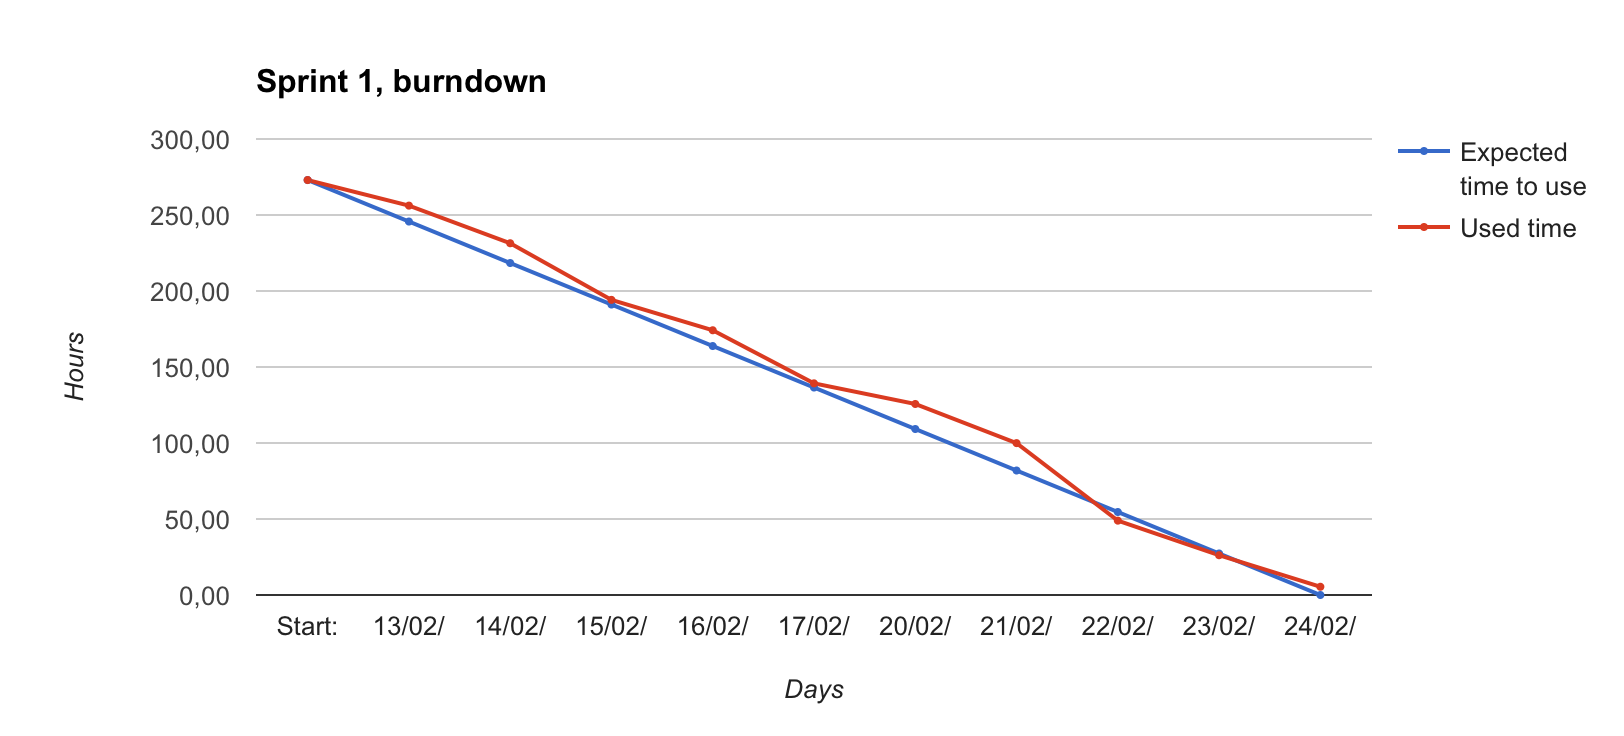
\includegraphics[width=0.8\textwidth]{fig/sprint1}
\caption{Sprint 1, burndown}
\end{figure}

\begin{figure}[ht]
\centering
    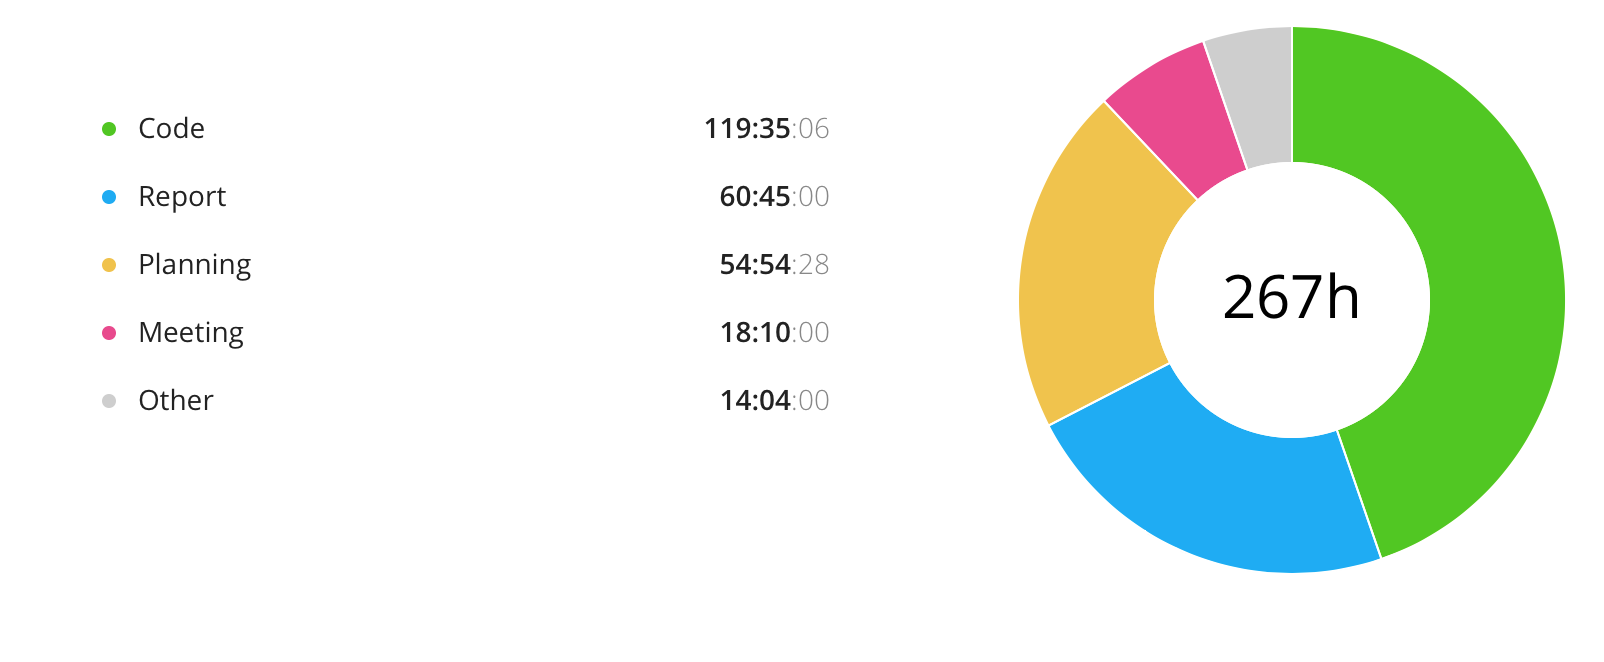
\includegraphics[width=0.8\textwidth]{fig/sprint1-diagram}
\caption{Sprint 1, hours distributed to work tasks}
\end{figure}
  

\section{Sprint 2} 
\label{sprint2}
The goal for sprint 2 was to implement functionality on the activities page; allowing the user to create and retrieve events, as well as filter these. The milestones in sprint 2 were as follows:

\begin{itemize}
  \item Log in.
  \item Fill database.
  \item Create events.
  \item Retrieve events.
  \item Filter events.
  \item Sign up for event.
\end{itemize}

The group experienced couple of problems during this sprint. Firstly, the group came across problems trying to implement the possibility to filter the activities. Initially the group had chosen to use flux to manage the data flow in the application. With further research and attempts trying to implement the flux pattern, the group realised it would not be sufficient in this project, as the application was required to support asynchronous actions. To solve this issue the group was required to complete further research on how this should be implemented, which consumed more of the sprint than first expected. Midway in the sprint the group decided to use Redux (see \ref{redux}) and research had to be completed on how this is implemented. Due to these issues the milestone, filter events, had to be relocated to sprint 3. 

During sprint 1 a set of milestones were defined and arranged after priority, which the group used to define the sprint backlogs. Midway in sprint 2 the customer arouse the desire for one of the final milestones, first version of release up and running on server, to be completed. To fulfill the customer's desire the group highly prioritized this milestone, which induced difficulties completing the original issues in the sprint backlog. To encounter this issue the group decided to re-prioritise the backlog subsequently after the request from the customer, moving the milestone at hand to sprint 2 and relocate the milestone "Sign up for activity" to sprint 3. 

Even tough the group encountered a couple of problems which affected what was included in the sprint backlog, and subsequently the sprint goal, the group was happy with what they had managed to accomplish. A lot of functionality was implemented and the group worked very well during this period. As an improvement to the upcoming sprints the group decided to become better at focusing on the issues in the sprint backlog, and not start developing functionality from the product backlog before the issues at hand were completed. 

\begin{figure}[ht]
\centering
    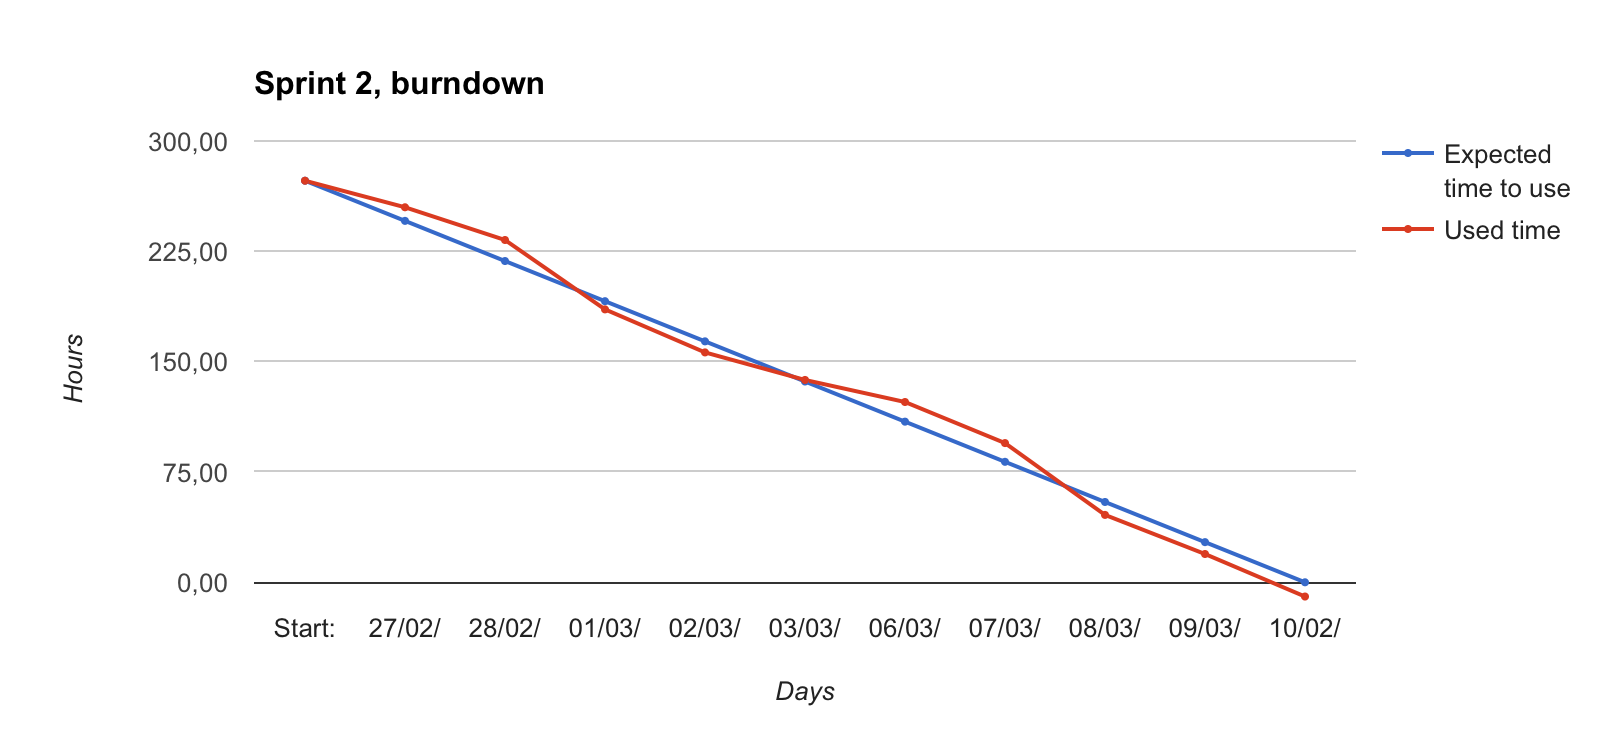
\includegraphics[width=0.8\textwidth]{fig/sprint2}
\caption{Sprint 2, burndown}
\end{figure}

\begin{figure}[ht]
\centering
    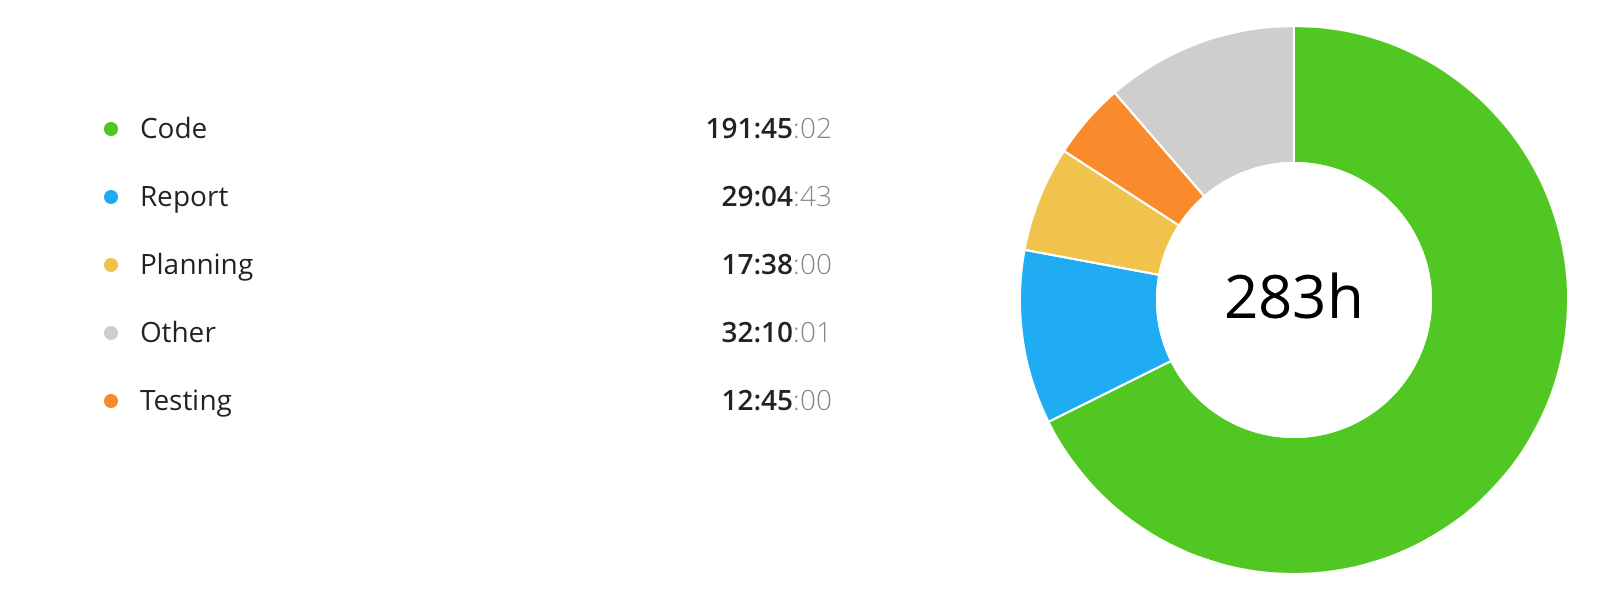
\includegraphics[width=0.8\textwidth]{fig/sprint2-diagram}
\caption{Sprint 2, hours distributed to work tasks}
\end{figure}

\section{Sprint 3}
\label{sprint3}
The main goal for this sprint was to implement user interaction with the events on the web portal. Two milestones from the previous sprint were also included in this sprint to be finalized. There was also a focus on making the web portal easy to install. The milestones were as as follows: 

\begin{itemize}
    \item Filter events (from sprint 2)
    \item Sign up for event (from sprint 2)
    \item Acceptance Tests
    \item Write User Test
    \item Loading bars
    \item My Page
    \item Create an installation for customer
    \item Create an installation guide
    \item Display active users in navigation bar
    \item Workshop
\end{itemize}

\begin{figure}[ht]
\centering
    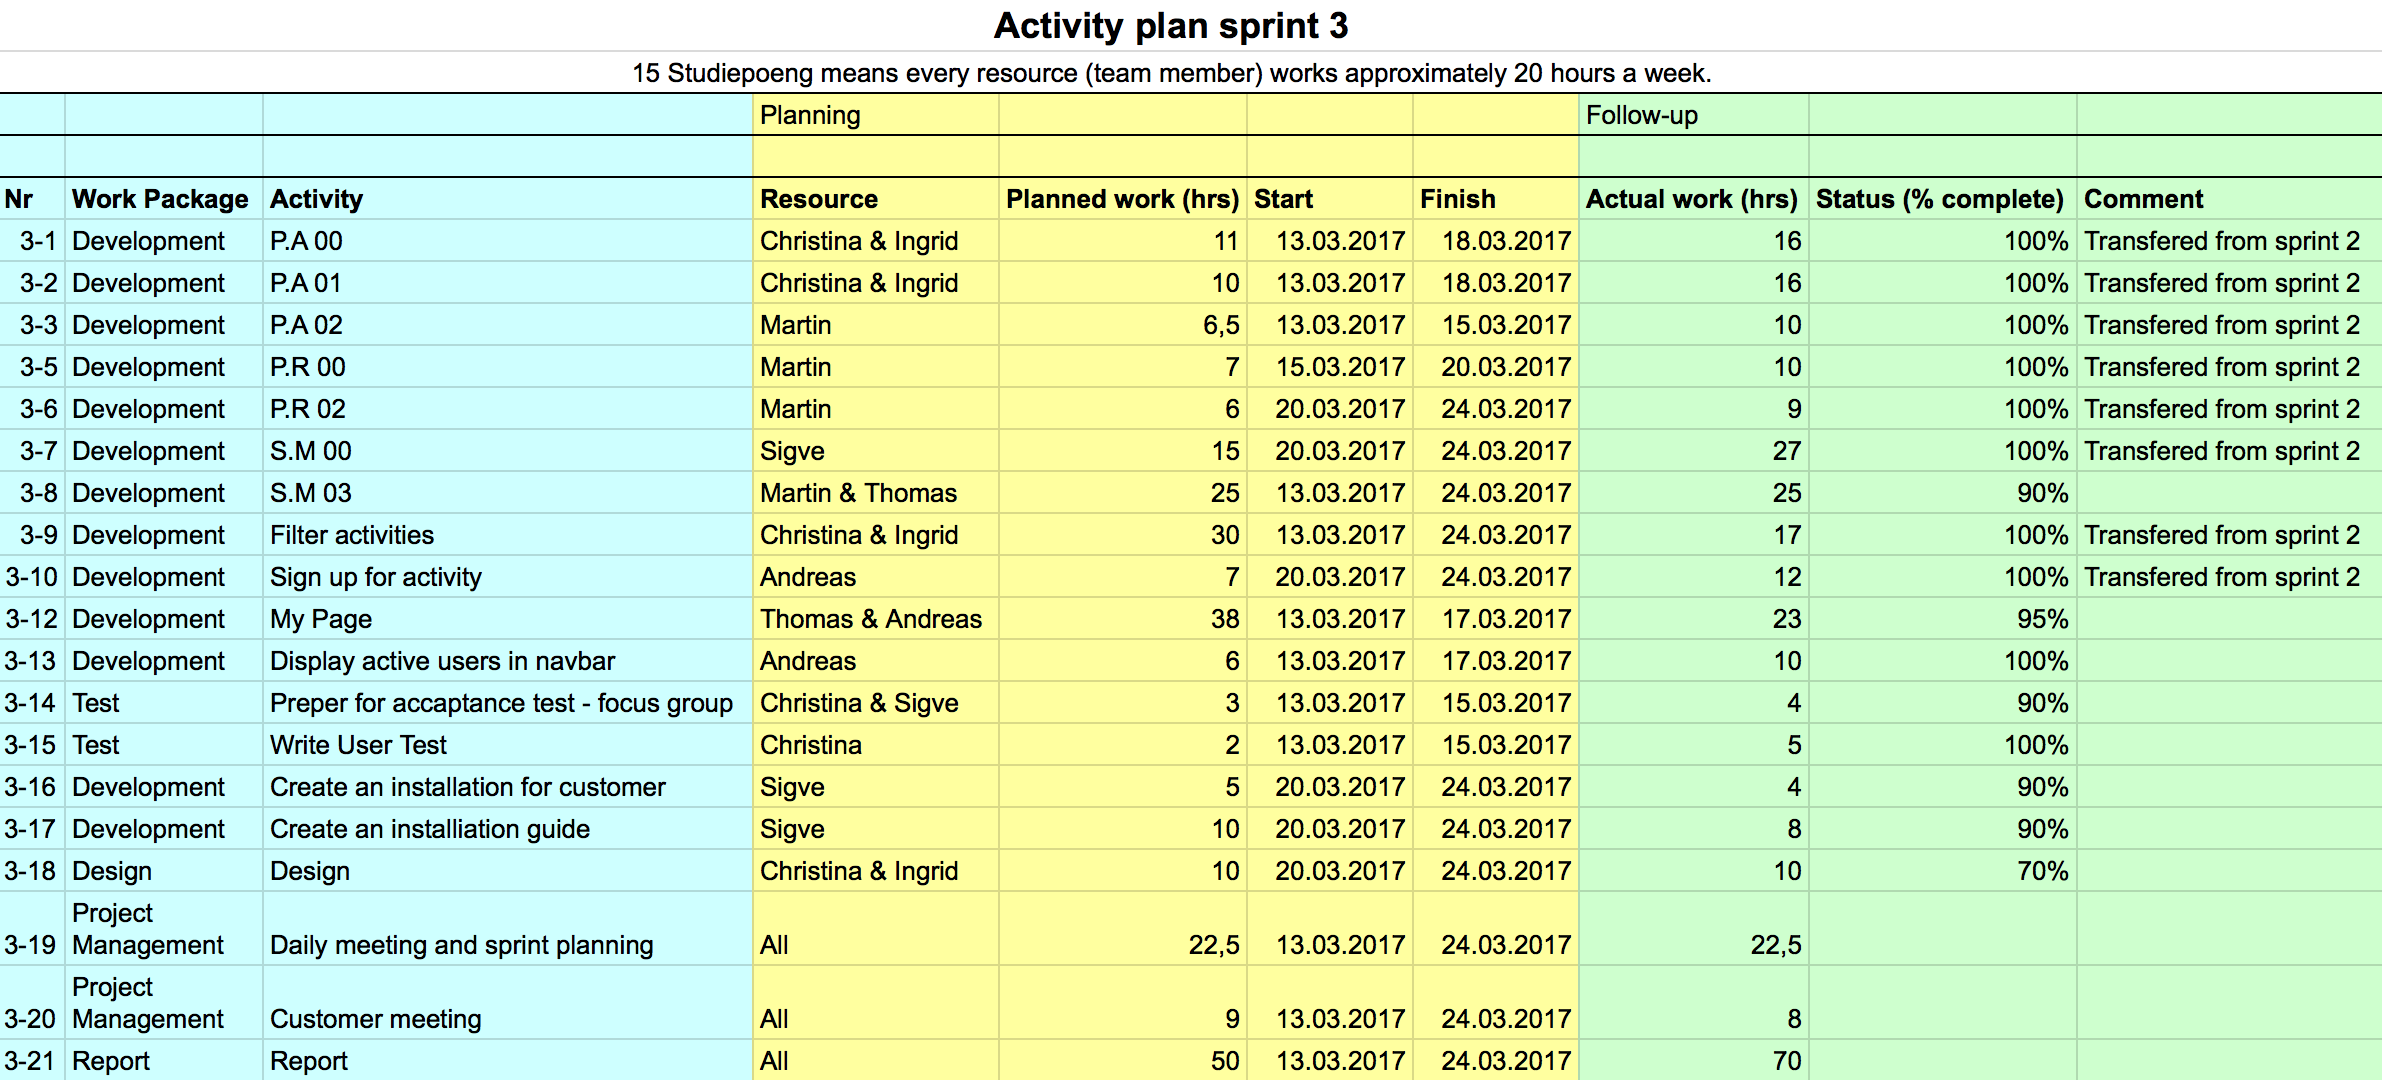
\includegraphics[width=\textwidth]{fig/activity_plan_3}
\caption{Activity Plan Sprint 3}
\end{figure}

The group was very effective this sprint and a lot of work were completed. No major problems were encountered and the minor problems were quickly resolved by asking the other team members for help.

In this sprint there was also made plans for conducting usability testing of the web portal. The test subjects were divided into two groups, one for system managers and the second for providers and users. While the web portal did not have any assigned system managers, providers or users, the selection was made based on whom was likely to fulfill this role in the future. This was accomplished by working together with the customer and arranging workshops. 

Because of schedules overlapping with the group and the customer, the workshops had to be postponed to the next sprints.

\begin{figure}[ht]
\centering
    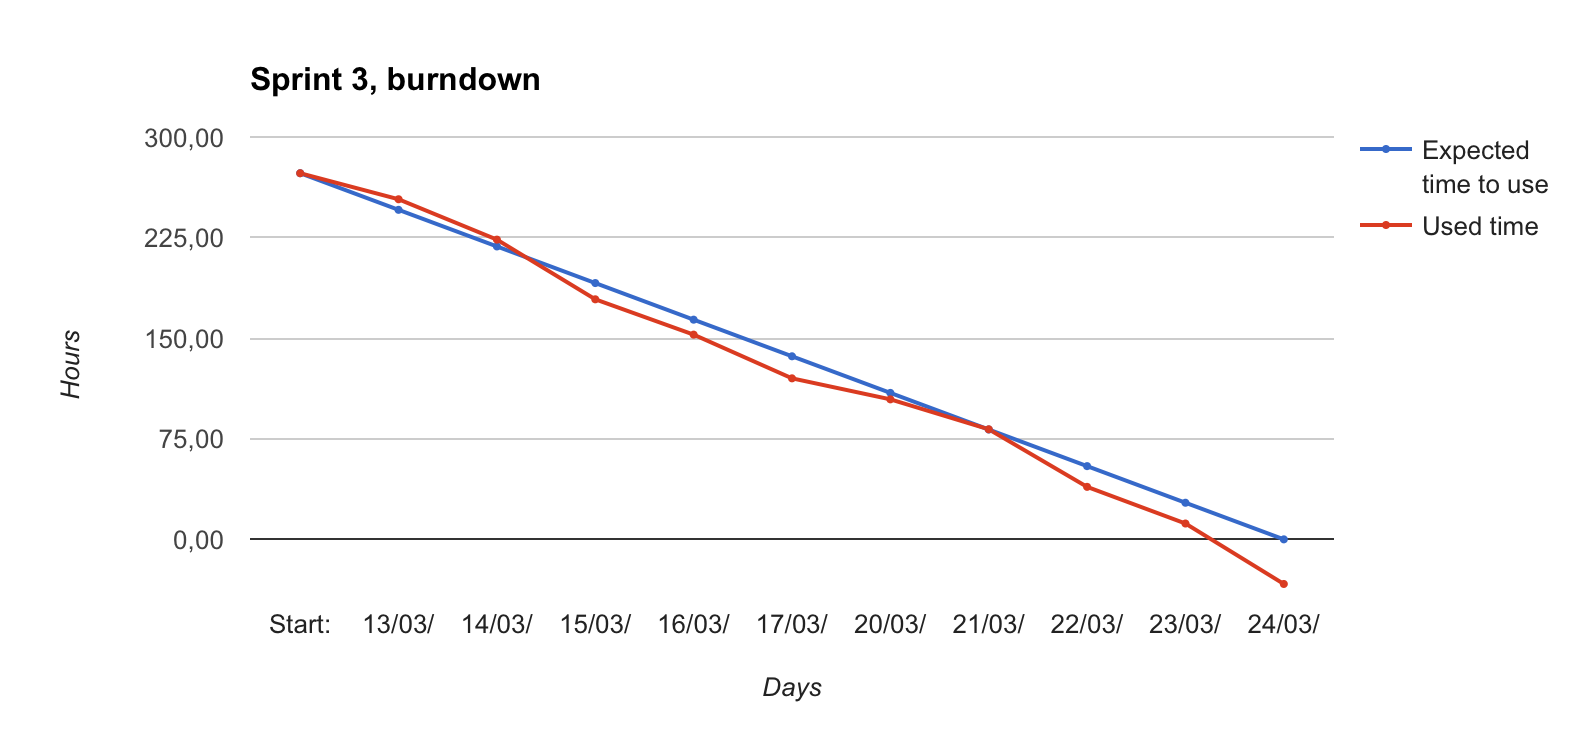
\includegraphics[width=0.8\textwidth]{fig/sprint3}
\caption{Sprint 3, burndown}
\end{figure}

\begin{figure}[ht]
\centering
    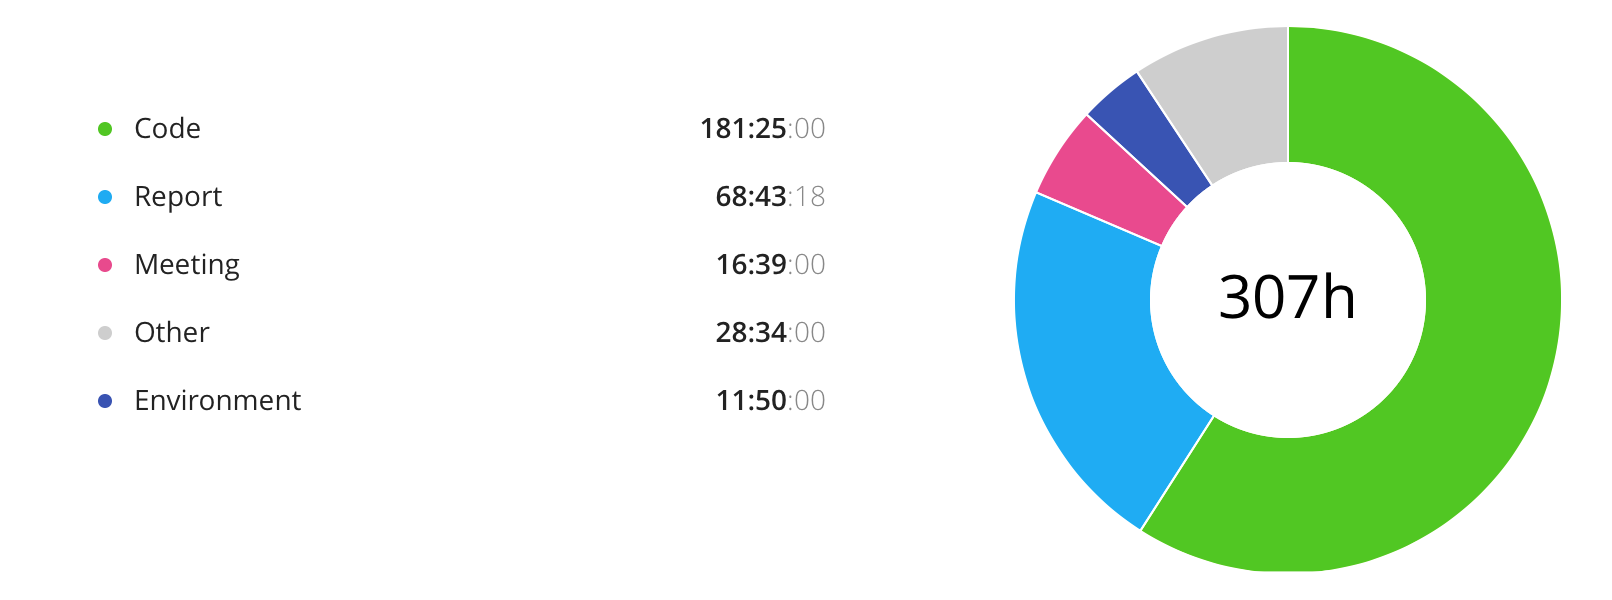
\includegraphics[width=0.8\textwidth]{fig/sprint3-diagram}
\caption{Sprint 3, hours distributed to work tasks}
\end{figure}

\section{Sprint 4 - Internal Feature Deadline}
\label{sprint4}
The main goal for this sprint was to implement and finalize the last product features, such as making it possible for a user to represent and see information about providers, and testing the web portal with through focus-groups.  

The feature milestones that were implemented and finalized during sprint 4 are listed below along with a short description and their relevant issue numbers on Github and Waffle.

\begin{itemize}
    \item Acceptance Test/focus-group test. \#54, 71, 
    \item Facebook sign in. \#112 
    \item Adaptions from DB, \#119,166, 201 
    \item Filter Activities \#161
    \item User represent provider, 
    \item Provider Page, \#167
    \item My Page, \#189
    \item easy Installation- and guide, \#53, S.M 00
    \item show assistent on activity. Note: P.A 04 done - removed later in sprint 5. Because of focusgroup family feedback.
\end{itemize}

\subsection{Sprint planning}
During the sprint planning, the group went through the product backlog once more and prioritized and re-estimated the workload. The group have previously decided that sprint four was the last sprint where the group could implement new and missing features. The last couple of weeks of the project could be used to clean up code, find and fix bugs and focus on documentation. 

The group discussed adding a new feature, robots.txt, which is a file that every search engine robot should check for existence, before indexing a web page. The feature was agreed upon, because of its low cost of implementation and its privacy boost. Robots.txt, is used to tell the web robots, not to index any images or other static information. This was done with the purpose of not letting the potential test data available in a Google search.

\begin{figure}[ht]
\centering
    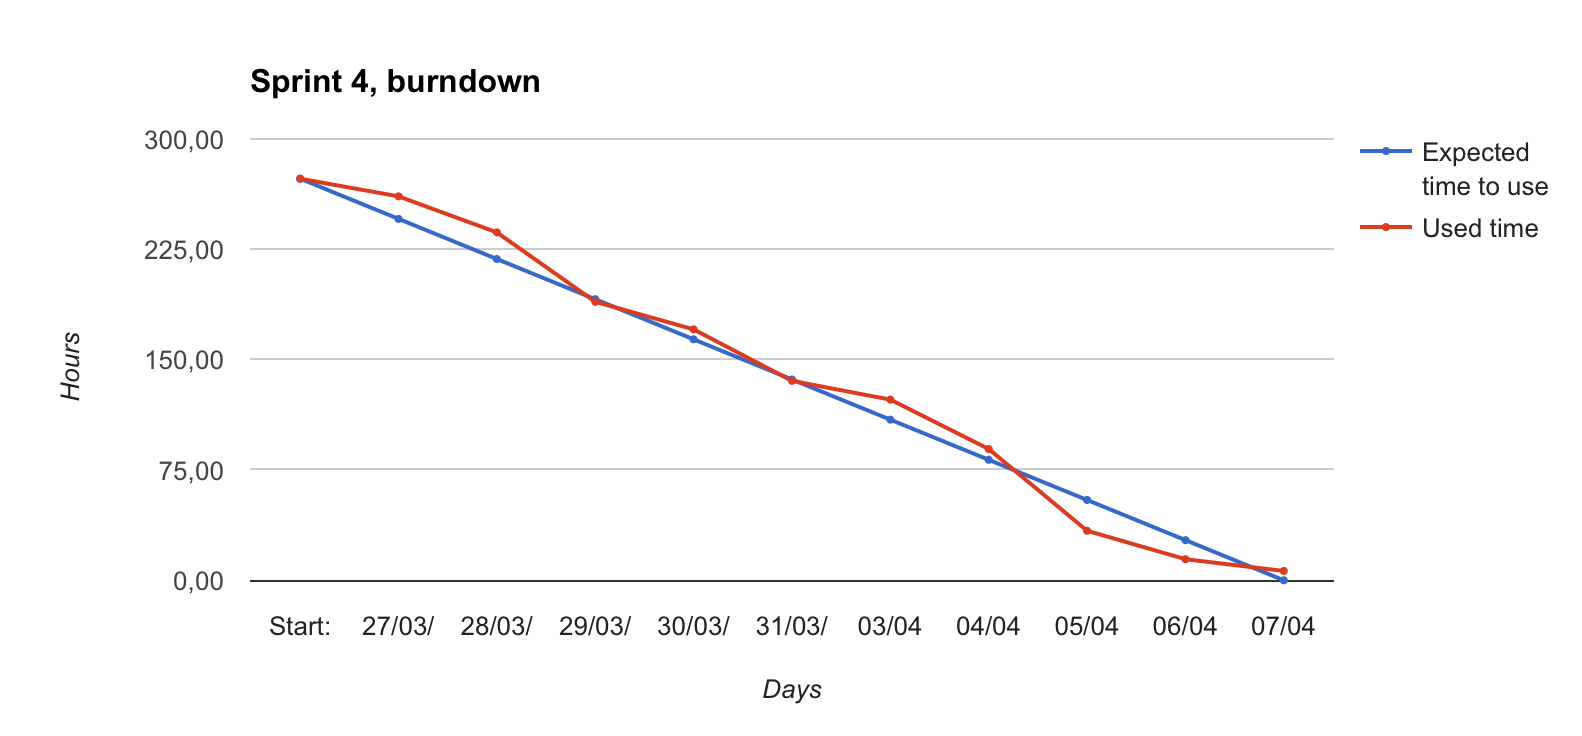
\includegraphics[width=0.8\textwidth]{fig/sprint4}
\caption{Sprint 4, burndown}
\end{figure}

\begin{figure}[ht]
\centering
    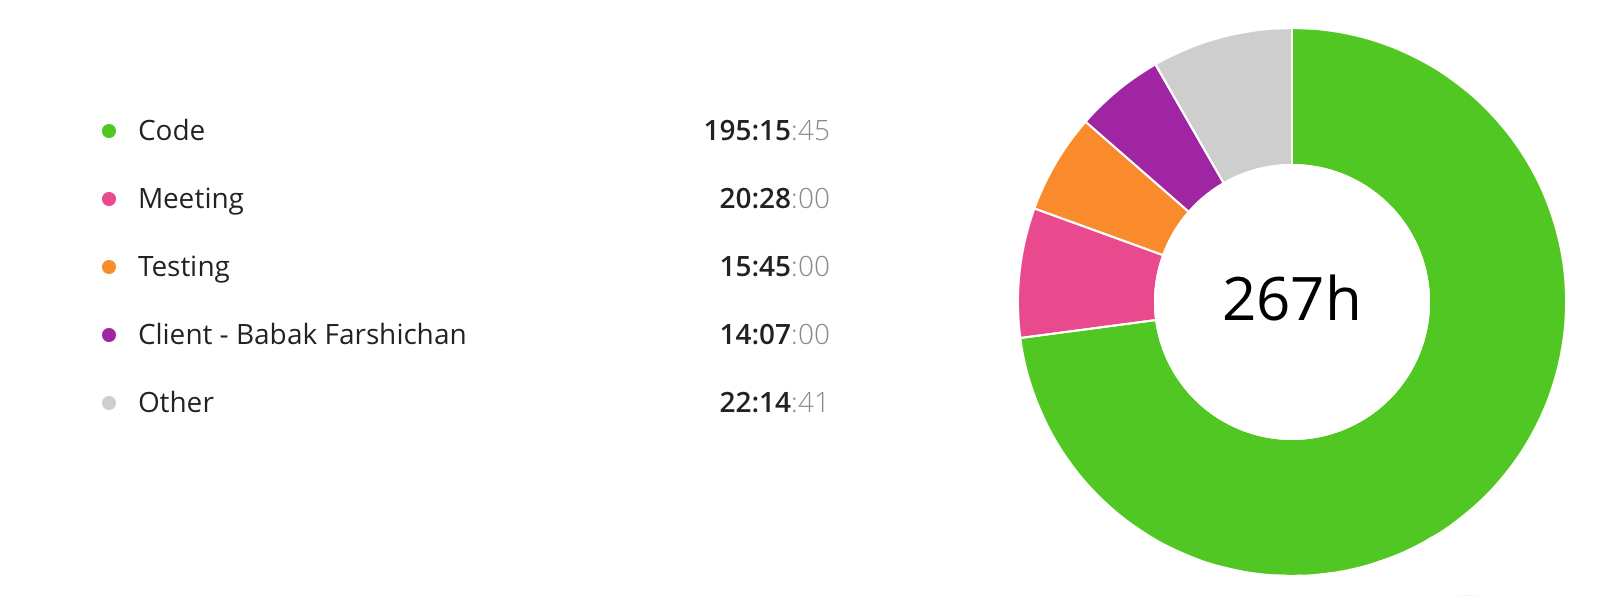
\includegraphics[width=0.8\textwidth]{fig/sprint4-diagram}
\caption{Sprint 4, hours distributed to work tasks}
\end{figure}

\subsection {Implementation and work}
The first thing that was finalized in sprint 4, was the easy installation and guide. The rest of the sprint went really well and there were none problems or other issues during the sprint, all features was implemented.

On the last sprint day, the group held a focus-group test with providers and possible system maintainers (see \ref{before_focus_group_with_providers}). Group members Skaugvoll and Norstein, represented and held the test on behalf of the group. The group demonstrated a few possible scenarios and the main concepts for providers and system maintainers, as well as for users. 
The response from customer, providers and system maintainers were that the concepts had a positive effect and that skalvi.no is heading in the right direction. They were surprised with how much the group have done and the state of web portal.

One question arise from the focus group, and was raised by one of  the providers. "Who will be administrators and owner of the web portal if it is to be taken further from "proof of concept" and into production?". The answer to this question is outside the scope of the group and in the hands of Sintef Digital and Trondheim Kommune.

\section{Sprint 5}
\label{sprint5}
This sprint was used to finalize the product and make it ready to deliver to the customer. It was therefore decided not to implement any new features, but to focus on the existing product and improve it. 

The workshop with the providers and users were also conducted during this sprint. Much time and effort where therefore put into preparing for the presentation and usability testing. 

After the workshop a group meeting was held to discuss the feedback. The feedback opened for many new ideas and constructive thoughts about the design. Later a meeting with the customer was held to discuss the feedback and the road ahead. 

At the end of the sprint the group went though all code produced and made sure it was well structured and readable. The information on Github was also updated so that the product could be delivered to the customer as complete as possible.


\begin{figure}[ht]
\centering
    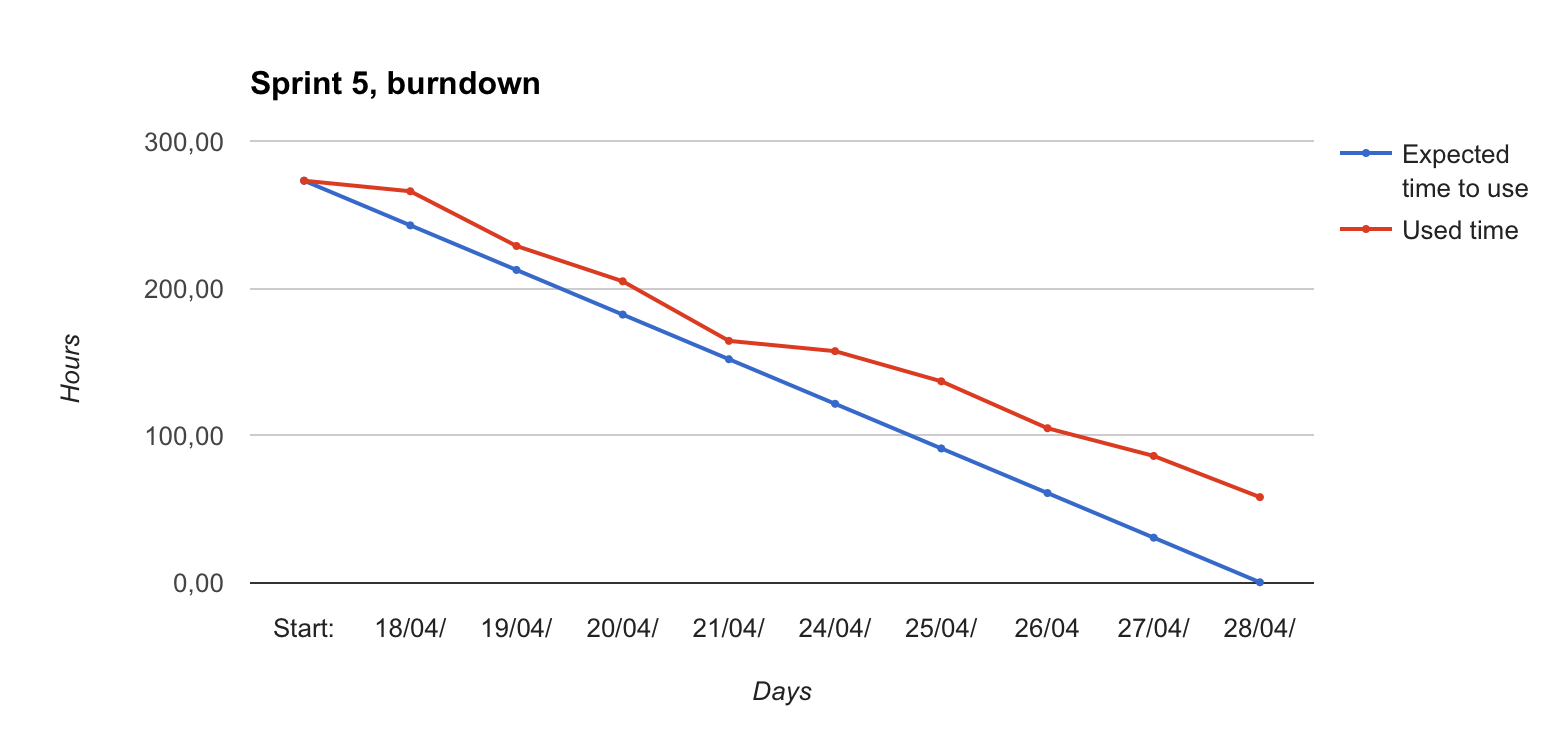
\includegraphics[width=0.8\textwidth]{fig/sprint5}
\caption{Sprint 5, burndown}
\end{figure}

\begin{figure}[ht]
\centering
    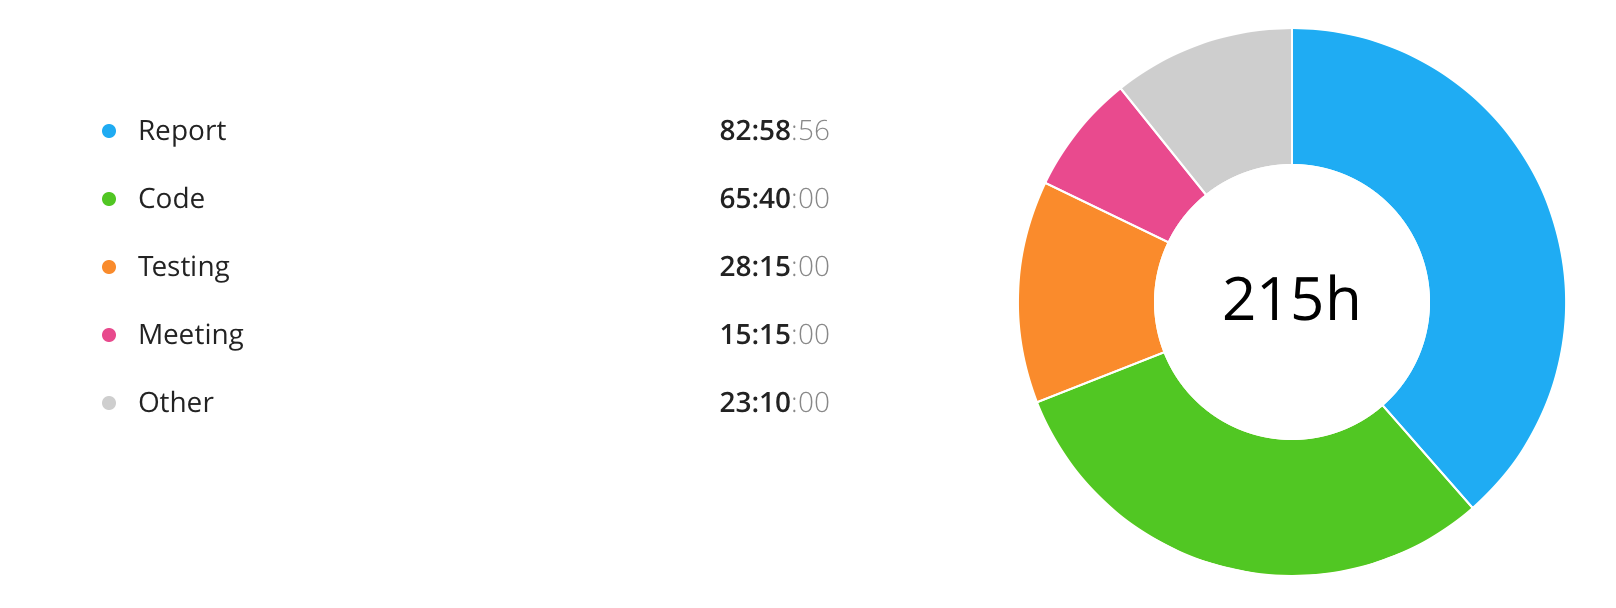
\includegraphics[width=0.8\textwidth]{fig/sprint5-diagram}
\caption{Sprint 5, hours distributed to work tasks}
\end{figure}

\cleardoublepage